\documentclass[../DoAn.tex]{subfiles}
\begin{document}
Chương này trình bày chi tiết về thiết kế phần mềm của hệ thống giám sát GNSS tích hợp. Mục tiêu của thiết kế là đảm bảo hệ thống hoạt động ổn định, hiệu quả và có khả năng thích ứng với môi trường hoạt động của các thiết bị IoT. Nội dung chương bao gồm kiến trúc tổng thể của phần mềm, mô hình phân lớp chức năng, mô tả chi tiết từng mô-đun chính và cơ chế tương tác giữa chúng. Ngoài ra, chương cũng tập trung vào các giải pháp tối ưu hiệu suất xử lý và tiết kiệm năng lượng, nhằm nâng cao độ tin cậy và kéo dài thời gian vận hành của thiết bị trong điều kiện thực tế. Các sơ đồ và bảng minh họa được sử dụng để hỗ trợ việc diễn giải kiến trúc và luồng dữ liệu trong hệ thống.
\section{Kiến trúc tổng thể phần mềm}
\label{section:4.1}
Phần mềm được thiết kế theo kiến trúc phân lớp nhằm đảm bảo tính mô-đun, dễ bảo trì và dễ mở rộng. Hệ thống được chia thành ba lớp chính: lớp giao tiếp phần cứng, lớp xử lý dữ liệu và lớp truyền thông - hiển thị.

Lớp giao tiếp phần cứng thực hiện việc thu thập dữ liệu từ thiết bị GNSS thông qua giao tiếp UART. Các byte dữ liệu được xử lý tuần tự để xây dựng các bản tin định vị hoàn chỉnh theo chuẩn NMEA và UBX.

Lớp xử lý dữ liệu chịu trách nhiệm phân tích, trích xuất và xác thực thông tin định vị từ các bản tin nhận được. Thông tin bao gồm toạ độ, tốc độ, trạng thái tín hiệu và các chỉ số liên quan đến chất lượng định vị. Lớp này cũng xử lý các thuật toán kiểm tra điểm nằm trong vùng địa lý (geofence), đồng thời lưu trữ dữ liệu vào bộ nhớ cục bộ trong trường hợp mất kết nối mạng.

Lớp truyền thông - hiển thị có chức năng gửi dữ liệu định vị và trạng thái thiết bị đến nền tảng ThingsBoard thông qua giao thức MQTT. Lớp này đồng thời tiếp nhận các cấu hình điều khiển từ máy chủ và cập nhật các thông số hoạt động tương ứng. Dữ liệu cũng được hiển thị trực tiếp trên giao diện ứng dụng người dùng để phục vụ giám sát thời gian thực.

Kiến trúc này cho phép phân tách rõ ràng giữa các chức năng, giảm thiểu sự phụ thuộc giữa các mô-đun, đồng thời hỗ trợ triển khai các cơ chế tối ưu tài nguyên và năng lượng phù hợp với đặc thù của thiết bị nhúng.
\begin{figure}[H]
    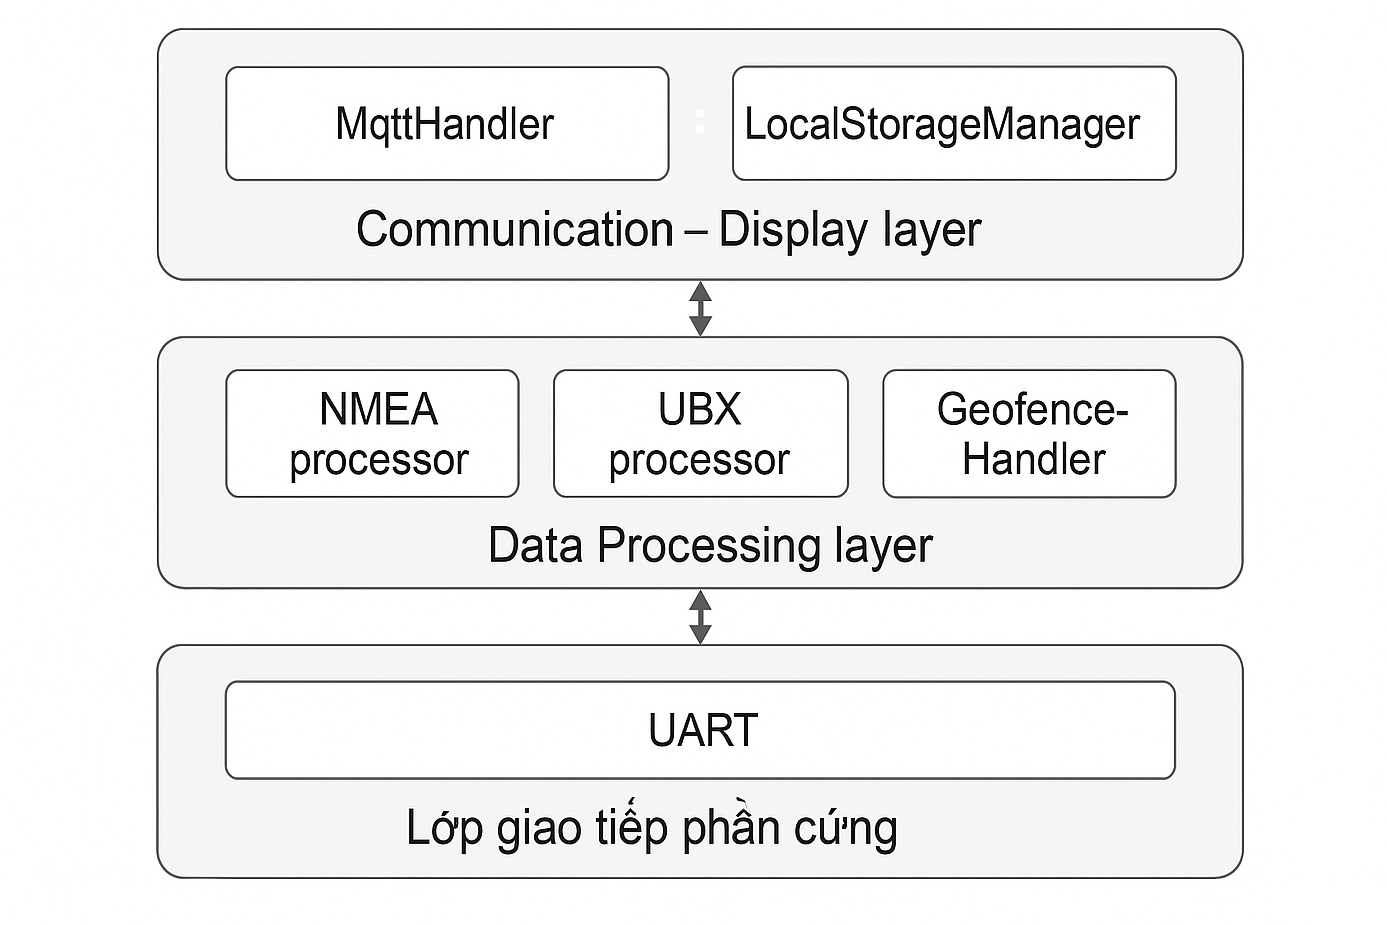
\includegraphics[width=\linewidth]{Hinhve/System.png}
    \caption{Kiến trúc tổng thể phần mềm}
    \label{fig:label}
\end{figure}

\section{Thiết kế phân lớp phần mềm}
\label{section:4.2}
\subsection{Lớp giao tiếp phần cứng}
\label{subsection:4.2.1}
Lớp giao tiếp phần cứng là lớp nền trong toàn bộ kiến trúc phần mềm, chịu trách nhiệm kết nối với thiết bị GNSS và thu nhận dữ liệu thông qua giao tiếp UART. Thành phần trung tâm trong lớp này là lớp \texttt{UartReader}, được xây dựng để thực hiện các thao tác mở cổng, đọc dữ liệu byte theo thời gian thực và gửi dữ liệu điều khiển xuống thiết bị.

Ngay khi thiết bị khởi động, ứng dụng sử dụng \texttt{UartReader} để mở cổng UART tại đường dẫn cấu hình sẵn (\texttt{/dev/ttyHSL0}). Nếu mở cổng thành công, một luồng xử lý riêng sẽ được kích hoạt để liên tục đọc từng byte từ thiết bị GNSS. Mỗi byte nhận được sẽ được chuyển vào chuỗi xử lý kế tiếp thông qua các lớp phân tích dữ liệu.

Luồng xử lý dữ liệu sau khi nhận byte từ UART được chia thành hai nhánh chính, tương ứng với hai định dạng bản tin phổ biến của thiết bị GNSS là NMEA và UBX. Nếu dữ liệu là bản tin NMEA, tức có ký tự bắt đầu là dấu \texttt{\$}, luồng byte sẽ được chuyển đến lớp \texttt{NMEAProcessor} để tái tạo thành một chuỗi hoàn chỉnh. Sau đó, chuỗi này được phân tích bởi lớp \texttt{NMEAHandler} nhằm trích xuất thông tin định vị như toạ độ, tốc độ di chuyển, hướng đi và tính hợp lệ của tín hiệu.

Ngược lại, nếu byte đầu là cặp \texttt{0xB5 0x62} thì dữ liệu thuộc định dạng UBX. Lúc này, nó sẽ được truyền đến các bộ xử lý như \texttt{GNSSProcessor}, \texttt{NavStatusProcessor} hoặc \texttt{SFRBXProcessor} để kiểm tra độ dài, xác thực checksum và phân tích phần nội dung payload. Các bộ xử lý này hỗ trợ việc trích xuất thông tin cấu hình GNSS hoặc trạng thái vệ tinh đang hoạt động.

Dữ liệu định vị hợp lệ sau khi được trích xuất sẽ được chuyển tiếp lên lớp xử lý trung gian để tính trung bình toạ độ, phát hiện ra các vi phạm geofence hoặc gửi thông tin đến nền tảng ThingsBoard thông qua giao thức MQTT. Bên cạnh chức năng đọc, lớp giao tiếp phần cứng còn cho phép gửi dữ liệu điều khiển xuống thiết bị GNSS. Chẳng hạn, lớp \texttt{GNSSControl} có thể tạo bản tin \texttt{UBX-CFG-GNSS} để bật hoặc tắt các hệ thống vệ tinh như GPS, GLONASS, Galileo hoặc BeiDou. Bản tin sau đó được gửi đi thông qua UART nhờ phương thức ghi của \texttt{UartReader}.

Luồng xử lý UART đảm bảo rằng dữ liệu GNSS được tiếp nhận liên tục và chính xác, bất kể trong điều kiện hoạt động bình thường hay gián đoạn mạng. Đây là bước đầu tiên và cũng là tiền đề quan trọng để hệ thống thực hiện các tác vụ giám sát, phân tích và truyền thông một cách ổn định, đáng tin cậy.
\begin{figure}[H]
    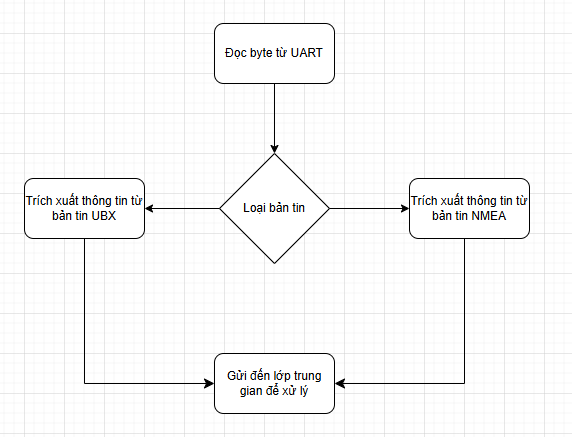
\includegraphics[width=\linewidth]{Hinhve/HardwareFlow.png}
    \caption{ Luồng xử lý dữ liệu lớp phần cứng}
    \label{fig:label}
\end{figure}
\subsection{Lớp xử lý dữ liệu}
\label{subsection:4.2.2}
Lớp xử lý dữ liệu đóng vai trò trung gian trong hệ thống, đảm nhận nhiệm vụ tiếp nhận dữ liệu thô từ lớp giao tiếp phần cứng, sau đó phân tích, trích xuất và xử lý thông tin định vị cần thiết. Lớp này được cấu trúc thành nhiều mô-đun chức năng, mỗi mô-đun đảm nhận một nhiệm vụ chuyên biệt tương ứng với các loại bản tin định vị khác nhau.
\subsubsection{Các bản tin từ module GNSS ublox NEO-M9}
\label{subsubsection:4.2.2.1}
Module GNSS u-blox NEO-M9 hỗ trợ truyền dữ liệu định vị qua hai định dạng bản tin chính là NMEA và UBX. Bản tin NMEA được sử dụng phổ biến để cung cấp thông tin vị trí dưới dạng chuỗi ASCII, trong khi bản tin UBX là định dạng nhị phân độc quyền của u-blox, cho phép truyền thông tin cấu hình và trạng thái với độ chính xác và linh hoạt cao hơn. Hệ thống phần mềm sử dụng bốn bản tin chính: \texttt{NMEA-RMC}, \texttt{UBX-CFG-GNSS}, \texttt{UBX-NAV-STATUS} và \texttt{UBX-RXM-SFRBX}, với chức năng và cấu trúc như sau:

Bản tin \texttt{RMC} (Recommended Minimum Specific GNSS Data) cung cấp thông tin tối thiểu cần thiết về định vị như thời gian, vị trí, tốc độ và hướng. Chuỗi bắt đầu bằng \texttt{\$GxRMC} và kết thúc bằng checksum. Các trường trong bản tin có định dạng văn bản, phân tách bằng dấu phẩy.

\begin{longtable}{|c|l|l|l|l|p{4cm}|}
\hline
\textbf{Field} & \textbf{Tên trường} & \textbf{Định dạng} & \textbf{Đơn vị} & \textbf{Ví dụ} & \textbf{Mô tả} \\
\hline
\endfirsthead

\hline
\textbf{Field} & \textbf{Tên trường} & \textbf{Định dạng} & \textbf{Đơn vị} & \textbf{Ví dụ} & \textbf{Mô tả} \\
\hline
\endhead

\hline
\endfoot

\endlastfoot

0 & xxRMC & Chuỗi & - & GPRMC & Mã tin nhắn RMC \\ \hline
1 & Thời gian & hhmmss.sss & - & 083559.00 & Thời gian UTC \\ \hline
2 & Trạng thái & Ký tự & - & A & Trạng thái tín hiệu (A = hợp lệ) \\ \hline
3 & Vĩ độ & ddmm.mmmm & Độ & 4717.11437 & Vĩ độ \\ \hline
4 & NS & Ký tự & - & N & Chỉ báo Bắc - Nam \\ \hline
5 & Kinh độ & dddmm.mmmm & Độ & 00833.91522 & Kinh độ \\ \hline
6 & EW & Ký tự & - & E & Chỉ báo Đông - Tây \\ \hline
7 & Tốc độ & float & knots & 22.4 & Tốc độ mặt đất \\ \hline
8 & Hướng đi & float & Độ & 84.4 & Hướng chuyển động \\ \hline
9 & Ngày & ddmmyy & - & 230394 & Ngày tháng năm \\ \hline
10 & mv & Số & Độ & - & Biến thiên từ trường \\ \hline
11 & mvEW & Ký tự & - & - & Biến thiên từ trường Đông - Tây \\ \hline
12 & posMode & Ký tự & - & A & Chỉ báo chế độ \\ \hline
13 & navStatus & Ký tự & - & V & Trạng thái định vị \\ \hline
14 & cs & Thập lục phân & - & 57 & Checksum \\ \hline
15 & CRLF & Ký tự & - & - & Ký tự xuống dòng \\ \hline

\caption{Cấu trúc bản tin NMEA-RMC} \\
\end{longtable}

Bản tin \texttt{UBX-CFG-GNSS} được sử dụng để cấu hình hệ thống GNSS đang hoạt động trên thiết bị. Bản tin chứa thông tin về số lượng kênh theo phần cứng và phần mềm, số hệ thống GNSS được cấu hình và trạng thái bật/tắt của từng hệ thống.

\begin{table}[H]
\centering
\begin{tabular}{|c|l|l|l|l|p{6cm}|}
\hline
\textbf{Offset} & \textbf{Tên trường} & \textbf{Định dạng} & \textbf{Đơn vị} & \textbf{Ví dụ} & \textbf{Mô tả} \\
\hline
0 & msgVer & uint8 & - & 0 & Phiên bản bản tin \\
\hline
1 & numTrkChHw & uint8 & kênh & 32 & Số kênh phần cứng hỗ trợ \\
\hline
2 & numTrkChUse & uint8 & kênh & 32 & Số kênh GNSS được sử dụng \\
\hline
3 & numConfigBlocks & uint8 & - & 6 & Số hệ thống GNSS được cấu hình \\
\hline
4 & repeated blocks & struct & - & ... & Dữ liệu cấu hình cho từng hệ thống GNSS (ID, số kênh, cờ enable, flags, v.v.) \\
\hline
\end{tabular}
\caption{Cấu trúc bản tin UBX-CFG-GNSS}
\end{table}

Bản tin \texttt{UBX-NAV-STATUS} cung cấp thông tin về trạng thái định vị hiện tại của thiết bị, bao gồm kiểu fix, các cờ trạng thái, và thông tin xác thực tín hiệu.

\begin{table}[H]
\centering
\begin{tabular}{|c|l|l|l|l|p{6cm}|}
\hline
\textbf{Offset} & \textbf{Tên trường} & \textbf{Định dạng} & \textbf{Đơn vị} & \textbf{Ví dụ} & \textbf{Mô tả} \\
\hline
0 & iTOW & uint32 & ms & 501867000 & Thời gian GPS (Time of Week) \\
\hline
4 & gpsFix & uint8 & - & 3 & Trạng thái định vị (3 = 3D fix) \\
\hline
5 & flags & bitfield & - & 0x0D & Các cờ phản ánh chất lượng và độ tin cậy tín hiệu \\
\hline
6 & fixStat & bitfield & - & 0x00 & Trạng thái xác định vị trí \\
\hline
7 & flags2 & bitfield & - & 0x00 & Các cờ bổ sung \\
\hline
\end{tabular}
\caption{Cấu trúc bản tin UBX-NAV-STATUS}
\end{table}

Bản tin \texttt{UBX-RXM-SFRBX} chứa dữ liệu thô từ tín hiệu vệ tinh, thường được sử dụng cho mục đích phân tích tín hiệu ở lớp thấp. Bản tin cung cấp thông tin như ID vệ tinh, tần số và các từ dữ liệu 32 bit từ mỗi vệ tinh.

\begin{table}[H]
\centering
\begin{tabular}{|c|l|l|l|l|p{6cm}|}
\hline
\textbf{Offset} & \textbf{Tên trường} & \textbf{Định dạng} & \textbf{Đơn vị} & \textbf{Ví dụ} & \textbf{Mô tả} \\
\hline
0 & gnssId & uint8 & - & 0 & ID hệ thống GNSS (0 = GPS) \\
\hline
1 & svId & uint8 & - & 3 & ID vệ tinh \\
\hline
2 & reserved1 & uint8 & - & 0 & Trường dự phòng \\
\hline
3 & freqId & uint8 & - & 0 & ID tần số tín hiệu \\
\hline
4 & numWords & uint8 & - & 10 & Số lượng từ dữ liệu GNSS \\
\hline
8 & dwrd & uint32[10] & - & ... & Dữ liệu 32 bit từ tín hiệu vệ tinh \\
\hline
\end{tabular}
\caption{Cấu trúc bản tin UBX-RXM-SFRBX}
\end{table}


\subsubsection{Luồng xử lý dữ liệu}
\label{subsubsection:4.2.2.2}
Lớp xử lý dữ liệu đóng vai trò trung gian trong hệ thống, đảm nhận nhiệm vụ tiếp nhận dữ liệu thô từ lớp giao tiếp phần cứng, sau đó phân tích, trích xuất và xử lý thông tin định vị cần thiết. Lớp này được cấu trúc thành nhiều mô-đun chức năng, mỗi mô-đun đảm nhận một nhiệm vụ chuyên biệt tương ứng với các loại bản tin định vị khác nhau.

Đối với dữ liệu NMEA, sau khi được tái dựng thành chuỗi hoàn chỉnh từ \texttt{NMEAProcessor}, chuỗi này sẽ được truyền vào lớp \texttt{NMEAHandler} để trích xuất các thông tin như vĩ độ, kinh độ, tốc độ di chuyển và trạng thái tín hiệu. Việc xử lý các câu lệnh \texttt{GGA}, \texttt{GNS}, \texttt{RMC}, hoặc \texttt{VTG} được thực hiện thông qua các parser chuyên biệt, giúp đảm bảo khả năng trích xuất chính xác từ đa nguồn GNSS.

Trong trường hợp bản tin có định dạng UBX, hệ thống sử dụng các mô-đun chuyên biệt như \texttt{GNSSProcessor}, \texttt{NavStatusProcessor} và \texttt{SFRBXProcessor}. Các mô-đun này thực hiện việc nhận diện chuỗi bản tin, kiểm tra độ dài hợp lệ, xác thực checksum và trích xuất thông tin cấu hình hoặc trạng thái vệ tinh. Thông tin này phục vụ cho việc xác định số lượng hệ thống GNSS đang hoạt động, theo dõi chất lượng tín hiệu hoặc tái cấu hình hoạt động GNSS thông qua các bản tin điều khiển.

Sau khi dữ liệu được phân tích và xác thực, lớp xử lý tiếp tục thực hiện các thao tác cao hơn như tính tốc độ di chuyển dựa trên thời gian thực và khoảng cách giữa các toạ độ, xác định thay đổi vị trí vượt quá ngưỡng cấu hình, hoặc phát hiện sự thay đổi trạng thái hoạt động của GNSS. Các dữ liệu hợp lệ được truyền đến lớp truyền thông để hiển thị hoặc đồng bộ với nền tảng giám sát.

Một chức năng quan trọng khác của lớp xử lý dữ liệu là hỗ trợ cơ chế geofence. Toạ độ được phân tích sẽ được kiểm tra thông qua lớp \texttt{GeofenceHandler}, sử dụng thuật toán kiểm tra điểm nằm trong đa giác để xác định xem thiết bị có nằm ngoài vùng giới hạn được cấu hình trước hay không. Kết quả này được sử dụng để gửi cảnh báo đến hệ thống khi có vi phạm ranh giới.

Ngoài ra, để đảm bảo hoạt động ổn định trong môi trường mạng không liên tục, các bản ghi dữ liệu định vị sẽ được lưu tạm thời bằng lớp \texttt{LocalStorageManager}. Khi mạng ổn định trở lại, dữ liệu này sẽ được đồng bộ qua lớp truyền thông MQTT. Cơ chế này giúp tránh mất dữ liệu trong quá trình thiết bị di chuyển qua các khu vực có chất lượng kết nối kém.

Toàn bộ lớp xử lý dữ liệu được thiết kế theo hướng mở rộng và tương thích với nhiều loại bản tin GNSS khác nhau, đảm bảo hiệu quả phân tích và tính linh hoạt trong các tình huống vận hành thực tế.
\subsection{Lớp truyền thông}
\label{subsection:4.2.3}
Lớp truyền thông có vai trò kết nối giữa thiết bị và nền tảng ThingsBoard thông qua giao thức MQTT. Thành phần trung tâm của lớp này là lớp \texttt{MqttHandler}, chịu trách nhiệm khởi tạo kết nối, gửi dữ liệu định vị, gửi các thông số trạng thái hệ thống và tiếp nhận các cấu hình điều khiển từ xa. 

Ngay khi khởi động, \texttt{MqttHandler} tiến hành kết nối đến máy chủ MQTT bằng định danh thiết bị ThingsBoard. Sau khi kết nối thành công, thiết bị sẽ tự động gửi một bản tin \texttt{init} chứa các thuộc tính cấu hình hiện tại của thiết bị.

Chương trình sử dụng hai topic chính: \texttt{telemetryTopic} để gửi dữ liệu thời gian thực như toạ độ và tốc độ di chuyển và \texttt{attributeTopic} để gửi hoặc nhận các thuộc tính cấu hình hệ thống như trạng thái pin, geofence hoặc điều kiện hoạt động. Tùy theo chế độ định vị, hệ thống sử dụng hai chế độ gửi dữ liệu:
\begin{itemize}
    \item \texttt{DEVICE\_LOCATION}: gửi tọa độ từ dịch vụ định vị của Android.
    \item \texttt{UBLOX\_LOCATION}: gửi tọa độ GNSS trung bình từ module u-blox.
\end{itemize}

Để tối ưu hiệu suất truyền thông và tiết kiệm năng lượng, lớp này chỉ gửi dữ liệu khi thiết bị có kết nối mạng hoặc khi tọa độ thay đổi vượt qua ngưỡng cấu hình. Nếu mất mạng, dữ liệu sẽ được lưu tạm thời trong bộ nhớ cục bộ thông qua lớp \texttt{LocalStorageManager} và tự động đồng bộ lại khi mạng ổn định trở lại.

Ngoài dữ liệu định vị, \texttt{MqttHandler} cũng xử lý các bản tin phản hồi từ ThingsBoard. Các bản tin thuộc chủ đề thuộc tính (\texttt{attribute}) được phân tích và cập nhật trực tiếp vào các thông số hoạt động như khoảng cách tối đa (\texttt{maxDistance}), thời gian tối đa (\texttt{maxTimeout}), tên tỉnh giám sát hoặc trạng thái bật/tắt vùng geofence. Nếu geofence được bật, ranh giới địa lý tương ứng với tỉnh được lấy từ file \texttt{provinces.json} và gửi ngược lên server để hiển thị trên dashboard.

Cuối cùng, lớp này còn hỗ trợ gửi các thuộc tính trạng thái như mức pin, trạng thái sạc, trạng thái GPS và cờ xác định thiết bị có nằm ngoài khu vực địa lý không (\texttt{isOutside}). Toàn bộ lớp được thiết kế bất đồng bộ, với cơ chế tự động kết nối lại khi xảy ra gián đoạn để đảm bảo tính liên tục trong quá trình truyền nhận dữ liệu.

\end{document}
